\section{Results}\label{sec:results}

To better understand the results, we performed an ANOVA analysis over all optimum values achieved from the GA-BBOB. These optimum values represent the values obtained from the 1728 different combinations paired by the 24 functions, the 3 dimensions and the 24 tournament sizes.

To get a finer intuition about these results, we show  some visual exemples separeted in two groups of Figures. The first group, shows the mean value achieved by the GA-BBOB given a function. The second one, shows the convergence plot with the mean of the values found at each generation, the function target value with a given tournament size.

All Figures represent the mean of 40 repetitions given a certain dimension.

\subsection{First Group}
The Figure~\ref{tournsizeF1} and the Figure~\ref{tournsizeF11} exemplify that for the F1 function (with 10 dimensions) and F11 (with 20 dimensions), that changing the tournament size, does not lead to significant better final values found by the GA-BBOB.


\begin{figure}[!ht]
	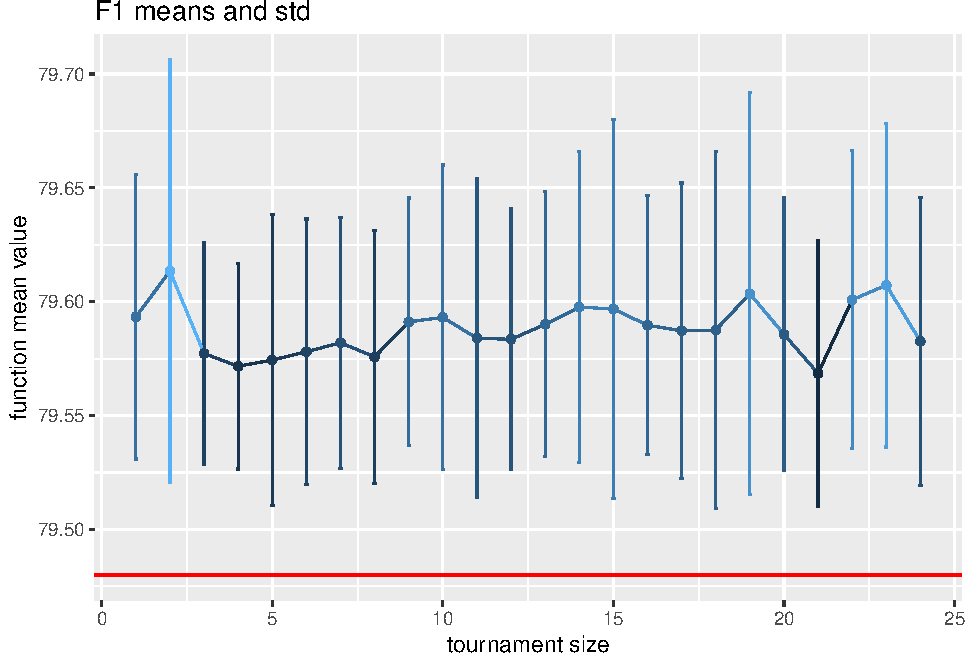
\includegraphics[width=0.45\textwidth]{img/pressure-1}
	\caption{Optimum values for the F1 function by the GA-BBOB. The mean of 40 repetitions is shown as bullets and the bars represent the standard deviation, with 10 dimensions.}
	\label{tournsizeF1}
\end{figure}

\begin{figure}[!ht]
	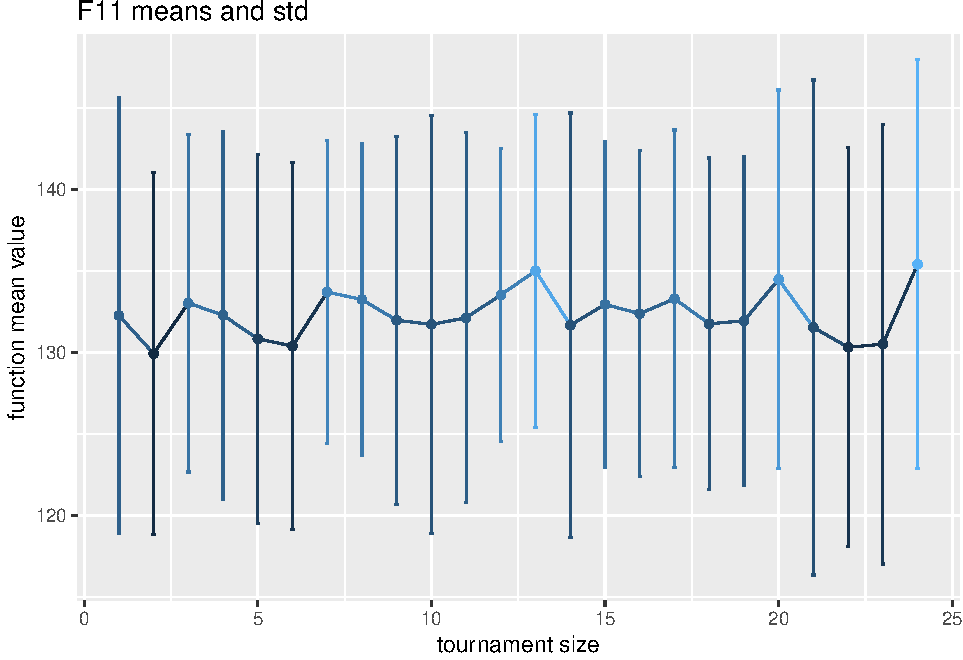
\includegraphics[width=0.45\textwidth]{img/pressure-21}
	\caption{Optimum values for the F11 function by the GA-BBOB. The mean of 40 repetitions is shown as bullets and the bars represent the standard deviation, with 20 dimensions.}
	\label{tournsizeF11}
\end{figure}

\subsection{Second Group}
The Figure~\ref{convegenceF1} exemplifies that for the F1 function (with 10 dimensions), the GA-BBOB is converging towards the optimum target value, represented by the red, vertical line. The same applies for the F11 function (with 20 dimensions), as is its possible to check on the Figure~\ref{convegenceF11}.

\begin{figure}[!ht]
	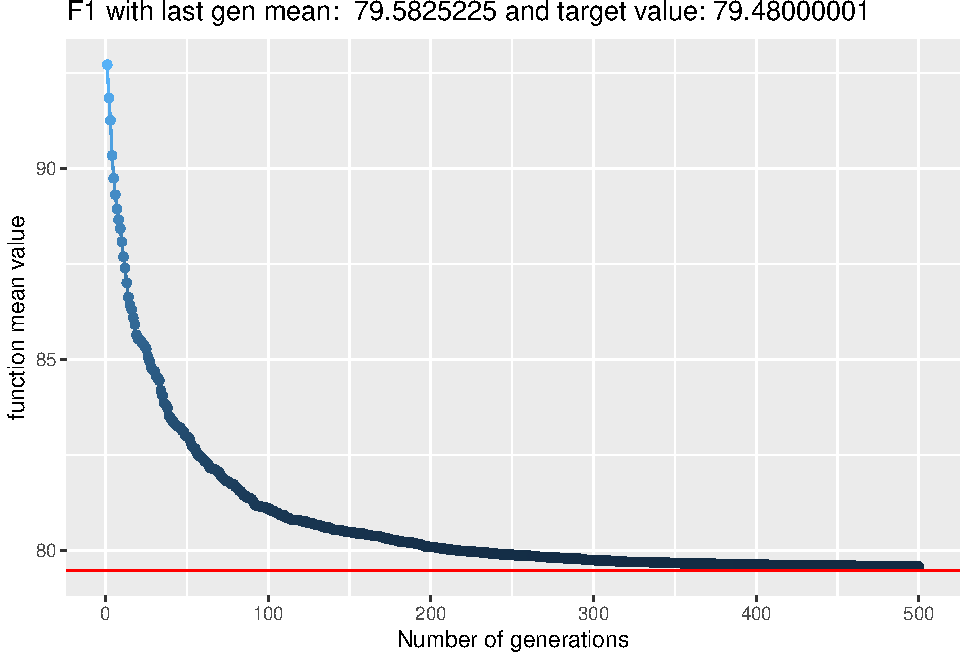
\includegraphics[width=0.45\textwidth]{img/unnamed-chunk-1-1}
	\caption{GA-BBOB population convergence for function F1. The mean of 40 repetitions is shown, with 10 dimensions.}
	\label{convegenceF1}
\end{figure}

\begin{figure}[!ht]
	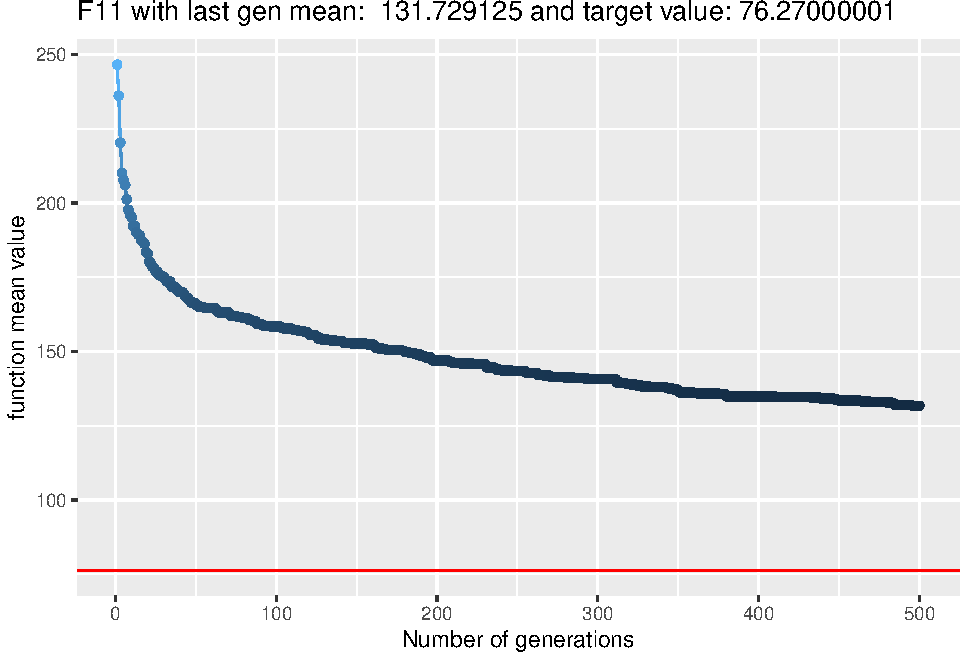
\includegraphics[width=0.45\textwidth]{img/unnamed-chunk-1-11}
	\caption{GA-BBOB population convergence for function F11. The mean of 40 repetitions is shown, with 20 dimensions.}
	\label{convegenceF11}
\end{figure}

\subsection{ANOVA}
The ANOVA analysis showed that, as expected,  number of dimensions, and e function were the variables that show some impact on the quality of the GA-BBOB outcome. Surprisingly enough,  no significant variation was found when comparing different tournament sizes. The data obtained from the ANOVA analysis can be seen (table/figure).